\documentclass[a4paper,11pt]{article}
\usepackage[T1]{fontenc}
\usepackage[utf8]{inputenc}
\usepackage[ngerman]{babel}
\usepackage{amssymb}
\usepackage{euler}
\usepackage{amsmath,amsthm}
\usepackage{enumerate}
\usepackage[inner=1.5in,outer=1in]{geometry}
\usepackage{todonotes}
\usepackage[ngerman,onelanguage,linesnumbered]{algorithm2e}
\usepackage{fancyhdr}
\usepackage{datetime}
\usepackage[noend]{algpseudocode}
\usepackage{caption,subcaption}
\usepackage{url}
\usepackage{csquotes}

\MakeOuterQuote{"}

\renewcommand{\bar}[1]{\overline{#1}}

\theoremstyle{definition}
\newtheorem{definition}{Definition}

\theoremstyle{plain}
\newtheorem{proposition}[definition]{Proposition}
\newtheorem{theorem}[definition]{Satz}
\newtheorem{lemma}[definition]{Lemma}
\newtheorem{corollary}[definition]{Korollar}

\theoremstyle{definition}
\newtheorem{bemerkung}[definition]{Bemerkung}
\newtheorem*{bemerkung*}{Bemerkung}

\newtheorem{claim}{Behauptung}
\renewcommand*{\theclaim}{\Alph{claim}}

\parskip=1ex
\parindent=0ex


\title{Einführung in \textit{Mechanism Design} \\ \Large im Seminar ``Algorithmische Spieltheorie''}
\author{Tim Greller}


\begin{document}

\maketitle

\begin{abstract}
	Dieses Handout gibt eine kurze Einführung in das Thema Mechanism Design. Dabei stellt der Designer Regeln auf, um möglichst effiziente und faire Ergebnisse zu erzielen. Es werden soziale Gruppenentscheidung für mehrere egoistische Spieler, basierend auf deren Präferenzen, getroffen. Soll diese Entscheidung möglichst nicht strategisch manipulierbar und nicht diktatorisch durch einen Spieler bestimmbar sein, so ist das im Allgemeinen nicht möglich. Um dem entgegenzuwirken und ein für die Allgemeinheit gutes Ergebnis zu erzielen, werden für die einzelnen Spieler Anreize durch Geld geschaffen.
\end{abstract}

\setcounter{page}{0}
\pagenumbering{arabic}
\fancyhead{}
\fancyhead[ER]{\leftmark}
\fancyhead[OL]{\rightmark}
\fancyhead[EL,OR]{\thepage}
\pagestyle{fancy}

\section{Einleitung, Definitionen}
Dieses Handout basiert auf dem Kapitel "Introduction to Mechanism Design (for Computer Scientists)" ~\cite{nis07}.

\emph{Mechanism Design} beschäftigt sich mit dem Aufstellen von Regeln um eine soziale Wahl zu erreichen. Diese soziale Wahl ist eine Gruppenentscheidung, die von den privaten Informationen der Spieler abhängig ist und sich auf alle Spieler auswirkt. Sie soll möglichst effizient für die Gemeinschaft ausfallen. Diesem Ziel steht allerdings das egoistische und unkooperative Verhalten der Spieler gegenüber: Ein Spieler unterstützt kein Ergebnis, wenn es nachteilig für ihn ist~\cite{ste08}.

Formal lässt sich die Entscheidung folgendermaßen betrachten:
Es gibt eine Menge $I$ an $n$-vielen \emph{Spielern}, die sich zwischen den \emph{Alternativen} $A$ entscheiden. Die Präferenzen zwischen den Alternativen stellen eine totale Ordnung von $A$ dar; Die Menge $L$ enthält alle dieser Ordnungen.

Eine \emph{Social Welfare Function} ist eine Funktion, die die Präferenzen aller Spieler zu einer einzigen, gemeinsamen Ordnung aggregiert. Im weiteren Verlauf bezeichnet $F$ immer eine Social Welfare Function.
\begin{definition}
	\label{def:socialwelfarefunc}
	Social Welfare Function $F : L^n \rightarrow L$
\end{definition}

\emph{Social Choice Functions} aggregieren die Präferenzen der Spieler zu einem einzigen, gemeinsamen Gewinner. Im weiteren Verlauf bezeichnet $f$ immer eine Social Choice Function.
\begin{definition}
	\label{def:socialchoicefunc}
	Social Choice Function $f : L^n \rightarrow A$
\end{definition}

\section{Vermeidung von Manipulation führt zur Diktatur}
\subsection{Arrow's Theorem bei Social Welfare Funktionen}
Zunächst werden Eigenschaften von $F$ betrachtet, die eine gute Social Welfare Funktion erfüllen sollte:
\begin{itemize}
	\item \emph{Einstimmigkeit} $\iff$ $\forall \prec \in L: F(\prec, \ldots,\prec) = \prec$
	\item \emph{Unabhängigkeit von irrelevanten Alternativen}
	$\iff$ $\forall a, b \in A; \prec_1,\ldots,\prec_n, \prec_1', \ldots, \prec_n' \in L:	(a\prec_i b \iff a\prec_i' b) \Rightarrow (a\prec b \iff a\prec' b)$	mit $\prec = F(\prec_1, \ldots, \prec_n)$, $\prec' = F(\prec_1', \ldots, \prec_n')$
\end{itemize}

Einstimmigkeit ist für ein $F$ erfüllt, wenn in dem Fall, dass alle Spieler mit einer gleichen, aber beliebigen Ordnung $\prec \in L$ abstimmen, das Ergebnis genau diese Ordnung ist. 

Die Unabhängigkeit von irrelevanten Alternativen (englisch: Independence of Irrelevant Alternatives, kurz: IIA) schließt strategisches Manipulieren aus. Gilt für $F$ IIA, so ist die soziale Präferenz für alle Alternativen $a, b \in A$ gleich, so lange auch die Präferenzen der Spieler bezüglich $a, b$ gleich sind. Die Präferenzen bzgl. aller anderen Alternativen untereinander und zu $a, b$ sind irrelevant.

Sucht man ein $F$, sodass diese beiden Eigenschaften erfüllt sind, existiert für alle $I, A, L$ die triviale Social Welfare Function $F(\prec_1, \ldots, \prec_n) = \prec_i$ mit einem beliebigen $i \in I$. Diese Funktion ist eine \emph{Diktatur}, da mit dem Spieler $i$ ein Diktator existiert. 

\begin{definition}
	\label{def:diktatur}
	$F$ ist Diktatur$\iff\exists i \in I: \forall \prec_1, \ldots, \prec_n \in L: F(\prec_1, \ldots, \prec_n) = \prec_i$
\end{definition}

Das soziale Ergebnis ist bei einer Diktatur also -- unabhängig von den Präferenzen anderer Spieler -- immer die Präferenz eines Spielers $i$.
Im folgenden wird bewiesen, dass dies ab $|A| > 2$ auch die einzige Lösung ist.

\begin{theorem}
	Alle Social Welfare Functions über mehr als 2 Kandidaten, die Einstimmigkeit und IIA erfüllen, sind Diktaturen. (Arrow's Theorem)
\end{theorem}

\begin{proof}
	Dieser Beweis basiert auf dem ersten der von John Geanakoplos vorgestellten Beweise~\cite{gea05}.
	
	\begin{claim} 
		\label{claim:extrementsch}
		Wenn bei einem Spielerprofil $\pi_0$ jeder Spieler eine Alternative $b$ je vor oder nach allen anderen platziert, so muss diese Alternative auch in der gemeinsamen Entscheidung $\succ = F(\pi_0)$ vor oder nach allen stehen.
	\end{claim}

	Angenommen dies gilt nicht. Dann existieren $a, c$, sodass $a \succ b \succ c$. Betrachte nun ein Profil $\pi_1$ in dem $c \succ_i' a$ und alles andere identisch zu $\pi_0$. Die Präferenzen zwischen $a, b$ und zwischen $a, c$ sind bei beiden Profilen gleich. Durch IIA folgt nun, dass $a \succ' b$ und $b \succ' c$. Transitiv gilt dadurch $a \succ' c$. Nach Definition von $\pi_1$ ist allerdings $c \succ_i' a$ $\forall i$ und daher durch Einstimmigkeit auch $c \succ' a$ -- ein Widerspruch.
	
	Betrachte nun die Profile $\pi_i^*$ mit $0 \leq i \leq n$ wobei die ersten $i$ Spieler $b$ an die vorderste Stelle und die letzten $n-i$ Spieler $b$ an die hinterste Stelle setzen. Die Alternative $b$ ist also nur an Extrempositionen vorzufinden. Dadurch muss $b$ laut Behauptung~\ref{claim:extrementsch} auch von der Social Welfare Funktion ganz vorne oder hinten angeordnet werden. Durch Einstimmigkeit gilt für $\pi_n^*$: $b \succ x$ $\forall x \in A$ und für $\pi_0^*$:  $x \succ b$ $\forall x \in A$. Dazwischen muss ein $\pi_{j-1}^*$ existieren, für das erstmalig $x \succ b$ gilt. Spieler $j$ kann in dieser Konstellation alleinig das soziale Ergebnis für $b$ entscheiden.
	
	\begin{claim}
		\label{claim:jdiktac}
		Der Spieler $j$ kann auch alleinig die Präferenz aller Paare $a,c$ mit $a, c \in I \setminus \{b\}$ entscheiden. Er ist Diktator über $a,c$.
	\end{claim}

	\begin{figure}
		\centering
		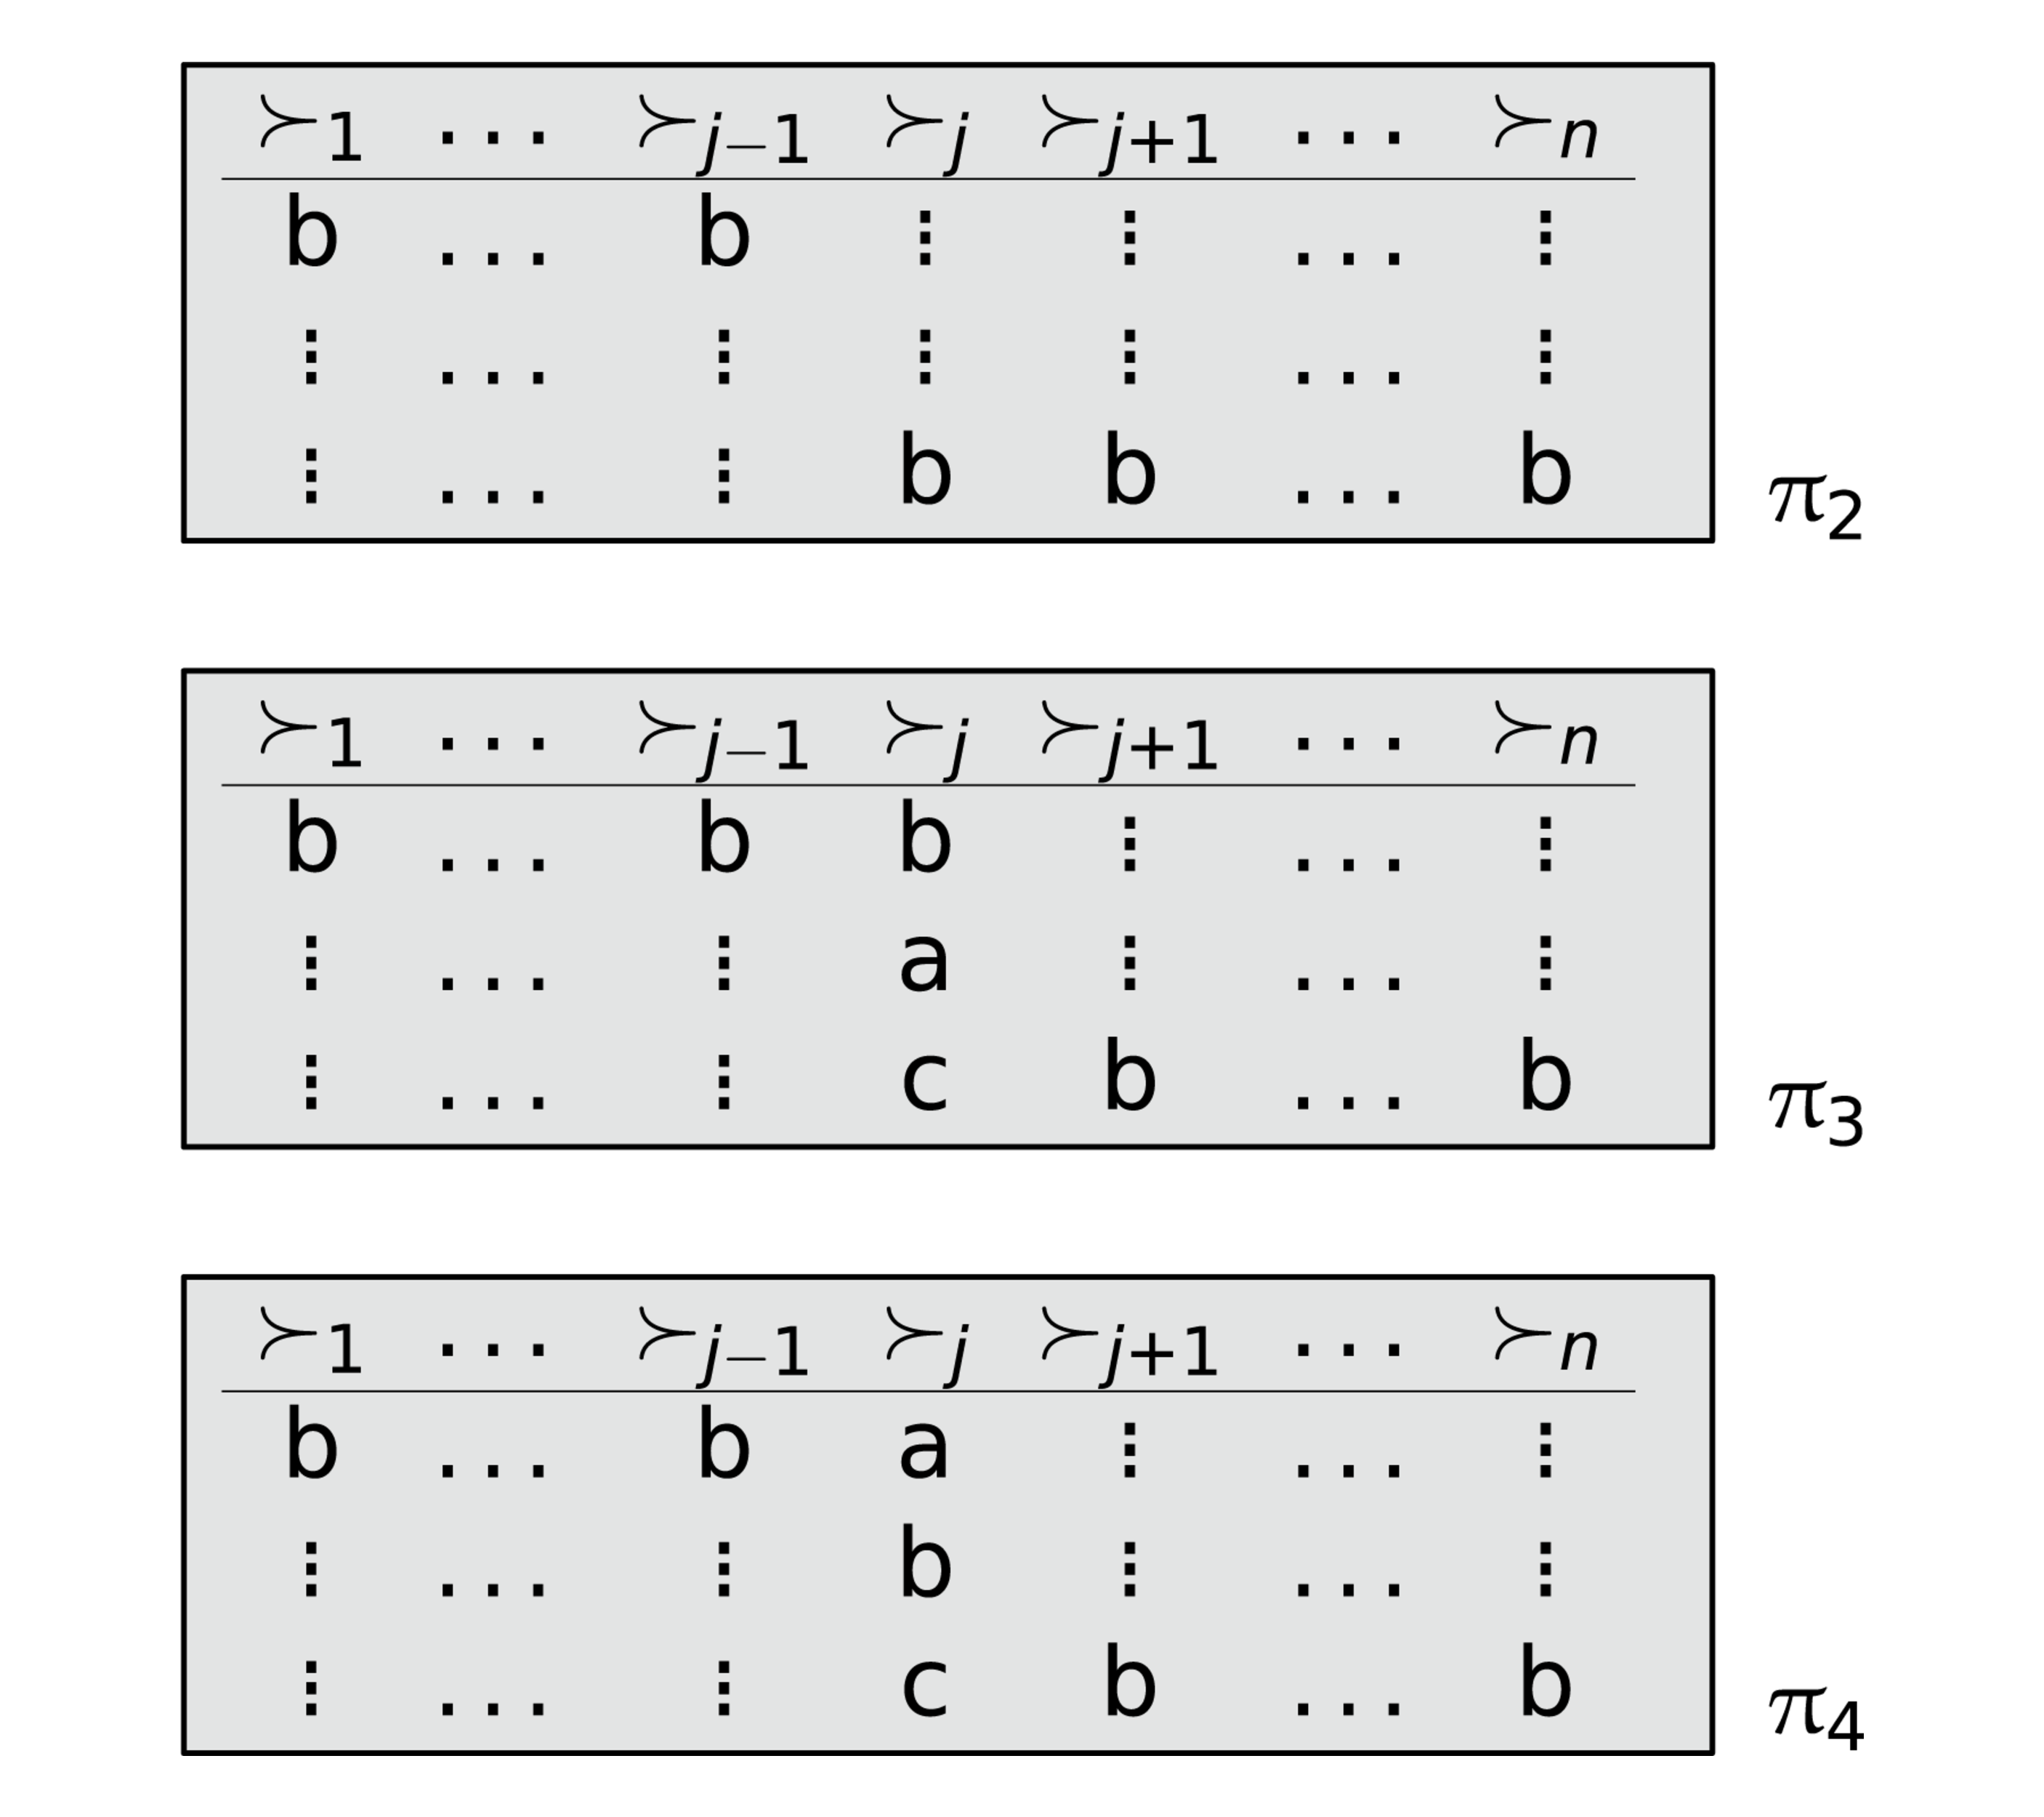
\includegraphics[width=.5\textwidth]{img/arrow(3).pdf}
		\caption{Beweis Arrow's Theorem: Spieler $j$ ist Diktator über alle Paare ohne $b$. Die abgebildeten Profile werden zum Zeigen dieser Aussage verwendet.}
		\label{fig:arr3}
	\end{figure}

	Dies wird gezeigt, indem ausgehend vom Profil $\pi_{j-1}^* =: \pi_2$ ein neues, identisches Profil $\pi_3$ (siehe Abbildung~\ref{fig:arr3}) erstellt wird, in dem Spieler $j$ die Alternativen $a,b,c$ neu anordnet und damit die Social Welfare Funktion zur gleichen Änderung zwingt.
	
	Da die $b$'s in $\pi_3$ wie bei $\pi_{j}^*$ positioniert sind, gilt $b \succ' x$ $\forall x \in I$ mit $\succ' = F(\pi_3)$. Zu zeigen ist nun, dass die Positionierung von $a$ über $c$ auch zu $a \succ' c$ führt. Gilt dies, kann durch Umbenennung allgemein gesagt werden, dass $j$ Kontrolle über alle Paare ohne $b$ hat.
	
	Hierzu werden $\pi_2$ und $\pi_3$ nun mit einem weiteren Profil $\pi_4$ verglichen. Dieses unterscheidet sich wieder nur bei Spieler $j$ von den vorherigen. In diesem Fall ordnet er $a$ über $b$ und $b$ über $c$ an. Analog zu den vorherigen Profilen sei $\succ'' = F(\pi_4)$. Da sich die Präferenzen von $I \setminus \{j\}$ nicht verändert haben und $a \succ_j b \iff a \succ_j'' b$ durch $x \succ_j b$ $\forall x \in I \Rightarrow a \succ_j b$ gilt, muss nach IIA auch $a \succ'' b$ gelten. Analog gilt durch $b \succ_j' c \iff b \succ_j'' c$ nach IIA auch $b \succ'' c$. Transitiv ergibt das $a \succ'' c$ und durch IIA gilt auch $a \succ' c$.
	
	
	
\end{proof}

\subsection{Gibbard-Satterthwaite bei Social Welfare Funktionen}
Analog zu Social Welfare Functions kann strategische Manipulation auch bei Social Choice Functions ausgeschlossen werden.
\begin{definition}
	\label{def:anreizkompatibel}
	$f$ ist \emph{anreizkompatibel}$\iff$$f$ nicht strategisch manipulierbar.
\end{definition}
Strategisch manipulierbar ist $f$, wenn für einen Spieler $i$, für $\prec_1, \ldots, \prec_n, \prec_i' \in L$ und $a = f(\prec_1, \ldots, \prec_i, \ldots, \prec_n)$, $a' = f(\prec_1, \ldots, \prec_i', \ldots, \prec_n)$ gilt: $a \prec_i a'$. In diesem Fall bevorzugt Spieler $i$ das Ergebnis $a'$, welches er durch taktisches Abweichen von seiner ursprünglichen Präferenz $\prec_i$ erreichen kann.

\section{Mechanism Design mit Geld}
\subsection{Vickrey's Second Price Auction}
\subsection{Vickrey-Clarke-Groves Mechanisms}
\subsection{Beispiel: Öffentliches Projekt, Clarke Pivot Rule}

\section{Bayesian-Nesh Implementation}
\subsection{First Price Auction}

\section{Zusammenfassung und Ausblick}
~\cite{lov21}

\bibliographystyle{alpha}
\bibliography{Literatur}

\end{document}
